% ==============================================================
% LIVE VIDEO STREAMER VIA NETWORK - TECHNICAL DOCUMENTATION
% Built using barebone_template.tex style
% ==============================================================

\documentclass[11pt,a4paper]{article}

% ============================================================
% PACKAGES
% ============================================================
\usepackage[utf8]{inputenc}
\usepackage[T1]{fontenc}
\usepackage{lmodern}
\usepackage[margin=1in]{geometry}
\usepackage{graphicx}
\usepackage{hyperref}
\usepackage{xcolor}
\usepackage{listings}
\usepackage{booktabs}
\usepackage{tabularx}
\usepackage{longtable}
\usepackage{amsmath}
\usepackage{amssymb}
\usepackage{bytefield}
\usepackage{fancyhdr}
\usepackage{titlesec}
\usepackage{enumitem}
\usepackage{tcolorbox}
\usepackage{float}
\usepackage{caption}
\usepackage{subcaption}
\usepackage{multicol}
\usepackage{tikz}
\usetikzlibrary{shapes,arrows,positioning,calc}

% ============================================================
% COLOR DEFINITIONS
% ============================================================
\definecolor{skyblue}{RGB}{0,102,204}
\definecolor{darkblue}{RGB}{0,51,102}
\definecolor{codebg}{RGB}{245,245,245}
\definecolor{codegreen}{RGB}{0,128,0}
\definecolor{codegray}{RGB}{128,128,128}
\definecolor{codepurple}{RGB}{128,0,128}
\definecolor{warnorange}{RGB}{255,140,0}
\definecolor{alertred}{RGB}{204,0,0}

% ============================================================
% HYPERREF SETUP
% ============================================================
\hypersetup{
    colorlinks=true,
    linkcolor=darkblue,
    urlcolor=skyblue,
    citecolor=darkblue,
    pdftitle={Live Video Streamer Technical Documentation},
    pdfauthor={Aadarsh Sinha and Krishnashis Das},
}

% ============================================================
% CODE LISTING STYLE (PYTHON & C)
% ============================================================
\lstdefinestyle{pythonstyle}{
    backgroundcolor=\color{codebg},
    basicstyle=\ttfamily\footnotesize,
    breaklines=true,
    captionpos=b,
    commentstyle=\color{codegreen},
    keywordstyle=\color{skyblue}\bfseries,
    stringstyle=\color{codepurple},
    numberstyle=\tiny\color{codegray},
    numbers=left,
    numbersep=5pt,
    frame=single,
    rulecolor=\color{codegray},
    language=Python,
    showstringspaces=false,
    tabsize=4,
    morekeywords={async,await,with,as,yield,True,False,None},
}
\lstset{style=pythonstyle}

% ============================================================
% HEADER / FOOTER
% ============================================================
\setlength{\headheight}{14pt}
\pagestyle{fancy}
\fancyhf{}
\fancyhead[L]{\textcolor{darkblue}{\textbf{Live Video Streamer v2.0}}}
\fancyhead[R]{\nouppercase{\leftmark}}
\fancyfoot[L]{\small \copyright\ Aadarsh Sinha and Krishnashis Das}
\fancyfoot[R]{\thepage}
\renewcommand{\headrulewidth}{0.4pt}
\renewcommand{\footrulewidth}{0.4pt}
\renewcommand{\sectionmark}[1]{\markboth{#1}{}}

% ============================================================
% CUSTOM TCOLORBOX ENVIRONMENTS
% ============================================================
\newtcolorbox{notebox}{colback=blue!5!white,colframe=skyblue,title=\textbf{Note},fonttitle=\bfseries}
\newtcolorbox{warnbox}{colback=orange!5!white,colframe=warnorange,title=\textbf{Warning},fonttitle=\bfseries}
\newtcolorbox{alertbox}{colback=red!5!white,colframe=alertred,title=\textbf{Security},fonttitle=\bfseries}

% ============================================================
% SECTION TITLE FORMATTING
% ============================================================
\titleformat{\section}{\Large\bfseries\color{darkblue}}{\thesection}{1em}{}
\titleformat{\subsection}{\large\bfseries\color{skyblue}}{\thesubsection}{1em}{}
\titleformat{\subsubsection}{\normalsize\bfseries\color{darkblue}}{\thesubsubsection}{1em}{}

% ==============================================================
% DOCUMENT BEGIN
% ==============================================================
\begin{document}

% ============================================================
% TITLE PAGE
% ============================================================
\begin{titlepage}
    \centering
    \vspace*{1.5cm}
    {\Huge\bfseries\textcolor{darkblue}{LIVE VIDEO STREAMER VIA NETWORK}\par}
    \vspace{0.4cm}
    {\Huge\bfseries\textcolor{skyblue}{FEATURE: INTERNET MODE}\par}
    \vspace{0.8cm}
    {\LARGE\textcolor{skyblue}{Version 2.0 Technical Specification}\par}
    \vspace{0.3cm}
    {\large\textcolor{codegray}{Cross-Network \& Zero-Configuration LAN Video Streaming}\par}
    \vspace{2cm}
    {\large Complete architectural, wire protocol, and implementation specification for high-throughput, low-latency live camera streaming over local networks and the public internet.\par}
    \vspace{2.5cm}

    {\normalsize
        \textbf{Author:} Aadarsh Sinha and Krishnashis Das\\
        GitHub Repository: \href{https://github.com/live-video-streamer}{\texttt{Live-video-streamer-via-network}}\\[1em]
        \textbf{Document Revision:} 2.0\\
        \vspace{0.8cm}
        \LARGE\textcolor{darkblue}{\textbf{System Specification \& Developer Guide}}
    }

    \vfill
    {\footnotesize\textcolor{codegray}{This document is an authoritative engineering specification. All client and server implementations must strictly conform to the 22-byte header framing and network rules defined herein.}}
\end{titlepage}

% ============================================================
% DOCUMENT CONTROL
% ============================================================
\newpage
\section*{Document Control}
\addcontentsline{toc}{section}{Document Control}

\begin{table}[H]
    \renewcommand{\arraystretch}{1.5}
    \begin{tabularx}{\textwidth}{@{}lX@{}}
        \toprule
        \textbf{Field} & \textbf{Value} \\
        \midrule
        \textbf{Document Title} & Live Video Streamer via Network (Internet Mode) Specification \\
        \textbf{Document ID}    & DOC-LVS-2026-V2 \\
        \textbf{Version}        & 2.0 \\
        \textbf{Status}         & Release Candidate / Final \\
        \midrule
        \textbf{Author(s)}      & Aadarsh Sinha and Krishnashis Das \\
        \textbf{Organization}   & Live Video Streamer Project \\
        \midrule
        \textbf{Release Date}   & \today \\
        \textbf{Last Updated}   & \today \\
        \midrule
        \textbf{Distribution}   & Open Source / Technical Public Specification \\
        \textbf{Classification} & \textcolor{darkblue}{\textbf{Technical Engineering Document}} \\
        \bottomrule
    \end{tabularx}
\end{table}

\vspace{1cm}

\begin{alertbox}
    \textbf{Protocol Version Compatibility Notice:} Version 2.0 introduces a 22-byte binary header with a \texttt{uint32} payload length field (\texttt{MAX\_PAYLOAD = 8 MB}). Version 1.0 clients (20-byte header with \texttt{uint16} payload length) are incompatible with Version 2.0 endpoints by design. Senders and receivers across the network must use identical protocol revisions to ensure clean packet parsing.
\end{alertbox}

% ============================================================
% REVISION HISTORY
% ============================================================
\newpage
\section*{Revision History}
\addcontentsline{toc}{section}{Revision History}

\begin{longtable}{@{}p{1.5cm}p{2.5cm}p{3.5cm}p{6cm}@{}}
    \toprule
    \textbf{Version} & \textbf{Date} & \textbf{Author(s)} & \textbf{Changes} \\
    \midrule
    \endfirsthead

    \multicolumn{4}{c}%
    {{\tablename\ \thetable{} -- continued from previous page}} \\
    \toprule
    \textbf{Version} & \textbf{Date} & \textbf{Author(s)} & \textbf{Changes} \\
    \midrule
    \endhead

    \midrule
    \multicolumn{4}{r}{{Continued on next page}} \\
    \endfoot

    \bottomrule
    \endlastfoot

    1.0 & 2026-08-01 & Aadarsh Sinha \& Krishnashis Das & Initial specification of LAN P2P streaming and 20-byte wire header with \texttt{uint16} payload length. \\
    1.1 & 2026-08-15 & Aadarsh Sinha \& Krishnashis Das & Added CLI VPS Relay server (\texttt{relay\_server.py}) for manual cross-network routing. \\
    2.0 & \today & Aadarsh Sinha \& Krishnashis Das & Upgraded wire protocol to 22-byte header (\texttt{uint32} payload length for 720p/1080p high quality frames), added automated Cloudflare Quick Tunnel integration (\texttt{cloudflared\_tunnel.py}), embedded MJPEG HTTP server (\texttt{mjpeg\_server.py}), multi-view web dashboard, and WebSocket Global Bridge mode. \\
    \bottomrule
\end{longtable}

% ============================================================
% TABLE OF CONTENTS
% ============================================================
\newpage
\tableofcontents
\newpage

% ============================================================
% ABSTRACT
% ============================================================
\section*{Abstract}
\markboth{Abstract}{}
\addcontentsline{toc}{section}{Abstract}

The **Live Video Streamer via Network** project is a lightweight, high-performance, cross-platform video streaming framework designed to transmit real-time camera feeds between devices over local networks (LAN) and across the public internet without complex port-forwarding or manual NAT traversal configuration. 

Built on Python's asynchronous \texttt{asyncio} event loop and OpenCV hardware video capture, the application offers four main modes of execution:
\begin{itemize}[noitemsep]
    \item \textbf{LAN Direct Mode (GUI):} Direct peer-to-peer TCP streaming using a custom binary wire protocol.
    \item \textbf{Internet Mode (Cloudflare Quick Tunnel):} Automated creation of HTTPS public streaming endpoints using an embedded HTTP MJPEG server paired with zero-config Cloudflare Tunnels.
    \item \textbf{Global Bridge Mode (WebSocket Hub):} Full-duplex WebSocket tunneling allowing mobile apps (e.g., Android) and remote web browsers to push and receive video frames worldwide.
    \item \textbf{VPS Relay Mode (CLI):} Standalone, zero-dependency VPS relay server (\texttt{relay\_server.py}) for enterprise deployments behind strict firewalls.
\end{itemize}

This specification details the mathematical framing of the custom 22-byte binary wire protocol, memory backpressure strategies, asynchronous thread model, auto-download lifecycle of binary tools, security considerations, and empirical performance metrics.

\newpage

% ============================================================
% 1. INTRODUCTION
% ============================================================
\section{Introduction}

\subsection{Overview}
Modern real-time video transmission solutions often suffer from steep infrastructure requirements, mandatory user account creations, or complex network address translation (NAT) configuration. The **Live Video Streamer** system resolves these friction points by providing a unified, multi-platform desktop interface (\texttt{app.py}) paired with modular CLI components.

When running on local networks, the system operates as a zero-relay TCP server, transferring compressed JPEG frames directly between the camera PC (Sender) and viewing clients (Receivers). When devices operate across disparate networks (such as cellular data vs. home Wi-Fi), the system seamlessly elevates the connection using automated **Cloudflare Quick Tunnels** or **WebSocket Global Bridges**.

\begin{notebox}
    Both PCs run the exact same executable script (\texttt{app.py}). Selecting \textbf{"Share My Camera"} spins up the TCP server and optional tunnel daemon, while \textbf{"Watch Stream"} initializes the receiver client engine.
\end{notebox}

\begin{warnbox}
    In high-resolution streaming (e.g., 720p or 1080p), single JPEG frame sizes routinely range between 100 KB and 400 KB. The wire protocol must handle arbitrary payload sizes without crashing the transport layer or stalling the main UI event loop.
\end{warnbox}

\begin{alertbox}
    \textbf{Security Warning:} By default, raw TCP socket streams do not employ application-layer encryption. For public Internet streaming, users should enable \textbf{Internet Mode}, which leverages Cloudflare's TLS/HTTPS encryption layer automatically.
\end{alertbox}

\subsection{Design Goals}
\begin{enumerate}
    \item \textbf{Zero Configuration NAT Traversal:} Eliminate manual router port forwarding by embedding managed tunnel subprocesses.
    \item \textbf{Asynchronous Non-Blocking Execution:} Isolate video capture and heavy JPEG compression in thread pools while maintaining sub-millisecond event loop responsiveness.
    \item \textbf{Resilient Frame Dropping (Backpressure Mitigation):} Protect network sockets by discarding stale video frames when client write buffers exceed safe thresholds (\texttt{WRITE\_BUFFER\_LIMIT = 2 MB}).
    \item \textbf{Universal Browser Compatibility:} Provide an embedded HTML5 / CSS3 dashboard with multi-camera grid viewing capability for any standard browser.
\end{enumerate}

\newpage

% ============================================================
% 2. ARCHITECTURE
% ============================================================
\section{Architecture Overview}

\subsection{System Architecture}
The system is divided into modular layer components: camera capture, binary protocol serialization, network transport, tunnel management, and user interface representation. Figure~\ref{fig:architecture} illustrates the end-to-end data flow in Internet Mode.

\begin{figure}[H]
    \centering
    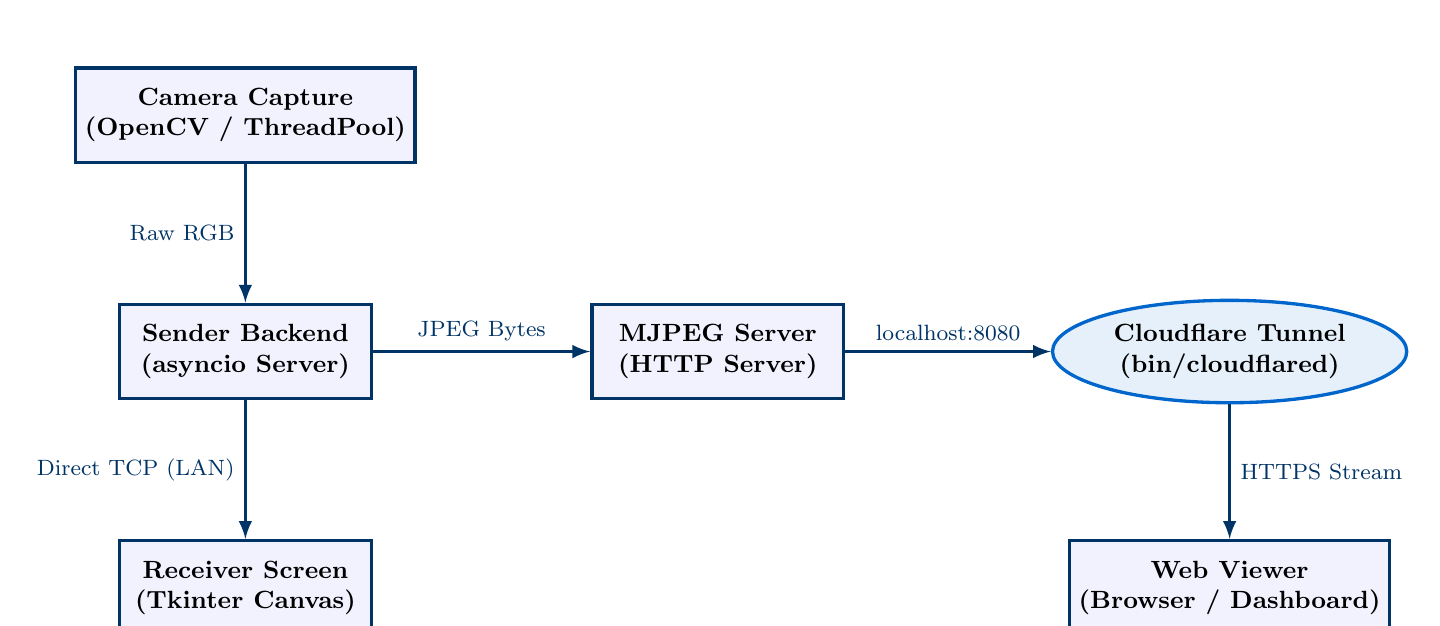
\begin{tikzpicture}[
        box/.style={rectangle, draw=darkblue, very thick, minimum width=3.2cm, minimum height=1.2cm, align=center, fill=blue!5, font=\small\bfseries},
        cloudbox/.style={ellipse, draw=skyblue, very thick, minimum width=3.0cm, minimum height=1.2cm, align=center, fill=skyblue!10, font=\small\bfseries},
        arrow/.style={->, very thick, >=latex, darkblue}]

        % Sender Nodes
        \node[box] (CAM) at (0,3) {Camera Capture\\(OpenCV / ThreadPool)};
        \node[box] (SND) at (0,0) {Sender Backend\\(asyncio Server)};
        \node[box] (MJPEG) at (6,0) {MJPEG Server\\(HTTP Server)};
        \node[cloudbox] (TUN) at (12.5,0) {Cloudflare Tunnel\\(bin/cloudflared)};
        
        % Viewer Nodes
        \node[box] (BROWSER) at (12.5,-3) {Web Viewer\\(Browser / Dashboard)};
        \node[box] (REC) at (0,-3) {Receiver Screen\\(Tkinter Canvas)};

        % Paths
        \draw[arrow] (CAM) -- node[midway, left, font=\footnotesize]{Raw RGB} (SND);
        \draw[arrow] (SND) -- node[midway, above, font=\footnotesize]{JPEG Bytes} (MJPEG);
        \draw[arrow] (MJPEG) -- node[midway, above, font=\footnotesize]{localhost:8080} (TUN);
        \draw[arrow] (TUN) -- node[midway, right, font=\footnotesize]{HTTPS Stream} (BROWSER);
        \draw[arrow] (SND) -- node[midway, left, font=\footnotesize]{Direct TCP (LAN)} (REC);

    \end{tikzpicture}
    \caption{System Architecture and Data Flow across LAN and Internet Modes}
    \label{fig:architecture}
\end{figure}

\subsection{Component Table}
\begin{table}[H]
    \centering
    \begin{tabularx}{\textwidth}{@{}lX@{}}
        \toprule
        \textbf{Module File} & \textbf{Functional Description} \\
        \midrule
        \texttt{app.py} & Unified Tkinter GUI application hosting Home, Sender, Receiver, and Multi-Bridge screens. \\
        \texttt{protocol.py} & Shared binary wire protocol serialization, header packing/unpacking, and timing helpers. \\
        \texttt{cloudflared\_tunnel.py} & Subprocess lifecycle manager for Cloudflare Quick Tunnel binary (auto-download \& health check). \\
        \texttt{mjpeg\_server.py} & Multi-threaded HTTP server providing standard \texttt{multipart/x-mixed-replace} MJPEG streams. \\
        \texttt{relay\_server.py} & Standalone \texttt{asyncio} VPS relay server for CLI-mode streaming across NAT networks. \\
        \texttt{sender.py} & Headless CLI camera publisher for servers and headless single-board computers. \\
        \texttt{receiver.py} & Headless CLI stream receiver and video playback handler. \\
        \texttt{mediamtx\_tunnel.py} & Alternative RTSP/RTMP/WebRTC tunnel manager using MediaMTX binary engine. \\
        \texttt{pinggy\_tunnel.py} & SSH-based tunnel backend for Pinggy port-forwarding fallback. \\
        \bottomrule
    \end{tabularx}
    \caption{Core System Module Overview}
\end{table}

\subsection{Thread \& Async Execution Model}
To prevent UI freezing during camera acquisition and frame encoding:
\begin{itemize}[noitemsep]
    \item \textbf{UI Thread (Tkinter):} Manages window events, button clicks, status dot updates, and renders RGB frames to a \texttt{tk.Label} canvas using \texttt{ImageTk.PhotoImage}.
    \item \textbf{Asyncio Loop Thread:} Operates a dedicated background \texttt{asyncio} event loop handling TCP client connection handshakes, PING/PONG heartbeats, and non-blocking socket writes.
    \item \textbf{ThreadPoolExecutor:} Offloads blocking hardware calls (\texttt{cv2.VideoCapture.read()}) and CPU-intensive JPEG compression (\texttt{cv2.imencode()}) to isolate the network loop.
\end{itemize}

\newpage

% ============================================================
% 3. SPECIFICATION
% ============================================================
\section{Wire Format \& Protocol Specification}


\subsection{Message Types}
\begin{table}[H]
    \centering
    \begin{tabular}{@{}llp{8cm}@{}}
        \toprule
        \textbf{Hex Code} & \textbf{Constant Name} & \textbf{Payload Content / Direction} \\
        \midrule
        \texttt{0x01} & \texttt{MSG\_REGISTER\_SENDER} & UTF-8 encoded stream name string (Client $\rightarrow$ Relay). \\
        \texttt{0x02} & \texttt{MSG\_REGISTER\_RECEIVER} & UTF-8 encoded stream name string (Client $\rightarrow$ Relay). \\
        \texttt{0x03} & \texttt{MSG\_REGISTER\_OK} & Empty payload (Relay $\rightarrow$ Client confirmation). \\
        \texttt{0x04} & \texttt{MSG\_REGISTER\_FAIL} & UTF-8 error string (Relay $\rightarrow$ Client rejection). \\
        \texttt{0x05} & \texttt{MSG\_VIDEO\_FRAME} & Raw JPEG compressed image binary data. \\
        \texttt{0x06} & \texttt{MSG\_PING} & Empty payload keepalive query. \\
        \texttt{0x07} & \texttt{MSG\_PONG} & Empty payload keepalive response. \\
        \texttt{0x08} & \texttt{MSG\_PEER\_DISCONNECTED} & Empty payload notification that sender exited. \\
        \bottomrule
    \end{tabular}
    \caption{Protocol Message Type Identifiers}
\end{table}

\subsection{Binary Header Byte Diagram}
The exact bit layout of the 22-byte fixed header is structured as follows:

\begin{center}
\begin{bytefield}[bitwidth=1.1em]{32}
    \bitheader{0,7,8,15,16,23,24,31} \\
    \bitbox{16}{MAGIC (16 bits)} & \bitbox{8}{VERSION} & \bitbox{8}{MSG\_TYPE} \\
    \wordbox{1}{STREAM\_ID (32 bits)} \\
    \wordbox{1}{SEQ\_NUM (32 bits)} \\
    \wordbox{1}{TIMESTAMP\_MS High 32 bits} \\
    \bitbox{16}{TIMESTAMP\_MS Low 16 bits} & \bitbox{16}{PAYLOAD\_LEN High 16 bits} \\
    \bitbox{16}{PAYLOAD\_LEN Low 16 bits} & \bitbox{16}{PAYLOAD DATA \dots}
\end{bytefield}
\end{center}

\subsection{Handshake \& Connection Sequence}
Figure~\ref{fig:sequence} details the registration and video frame streaming sequence between a Sender, VPS Relay, and Receiver client.

\begin{figure}[H]
    \centering
    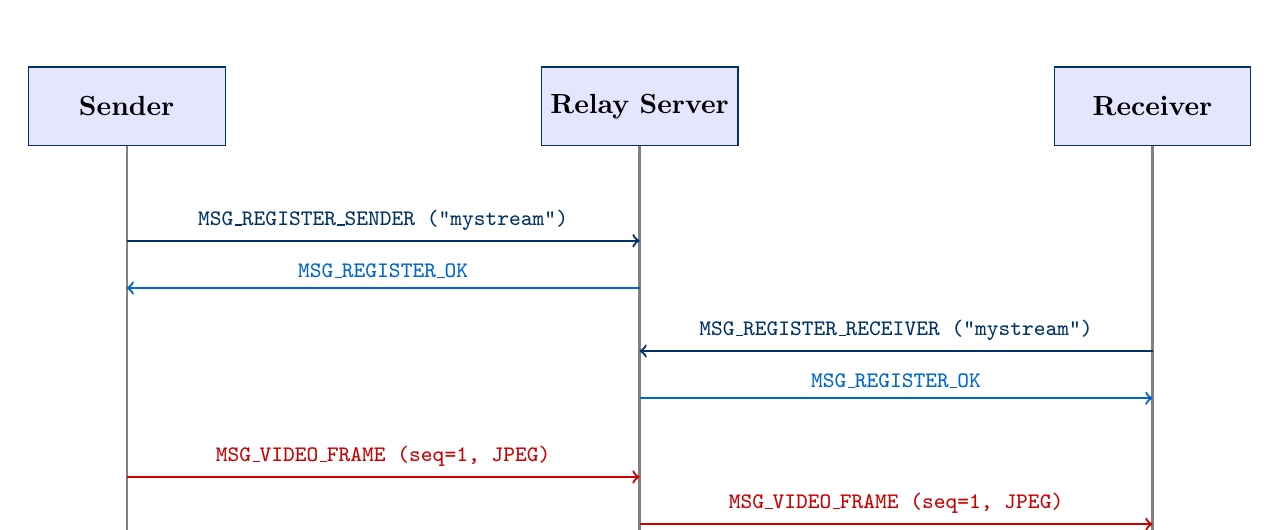
\begin{tikzpicture}[
        node distance=4cm,
        actor/.style={rectangle, draw=darkblue, fill=blue!10, minimum width=2.5cm, minimum height=1cm, font=\bfseries},
        line/.style={draw, thick, color=codegray}
    ]
        % Actors
        \node[actor] (SND) {Sender};
        \node[actor, right=of SND] (RLY) {Relay Server};
        \node[actor, right=of RLY] (RCV) {Receiver};

        % Lifelines
        \draw[line] (SND) -- ++(0,-5.5);
        \draw[line] (RLY) -- ++(0,-5.5);
        \draw[line] (RCV) -- ++(0,-5.5);

        % Messages
        \draw[->, thick, darkblue] ([yshift=-1.2cm]SND.south) -- node[above, font=\footnotesize]{\texttt{MSG\_REGISTER\_SENDER ("mystream")}} ([yshift=-1.2cm]RLY.south);
        \draw[->, thick, skyblue] ([yshift=-1.8cm]RLY.south) -- node[above, font=\footnotesize]{\texttt{MSG\_REGISTER\_OK}} ([yshift=-1.8cm]SND.south);

        \draw[->, thick, darkblue] ([yshift=-2.6cm]RCV.south) -- node[above, font=\footnotesize]{\texttt{MSG\_REGISTER\_RECEIVER ("mystream")}} ([yshift=-2.6cm]RLY.south);
        \draw[->, thick, skyblue] ([yshift=-3.2cm]RLY.south) -- node[above, font=\footnotesize]{\texttt{MSG\_REGISTER\_OK}} ([yshift=-3.2cm]RCV.south);

        \draw[->, thick, alertred] ([yshift=-4.2cm]SND.south) -- node[above, font=\footnotesize]{\texttt{MSG\_VIDEO\_FRAME (seq=1, JPEG)}} ([yshift=-4.2cm]RLY.south);
        \draw[->, thick, alertred] ([yshift=-4.8cm]RLY.south) -- node[above, font=\footnotesize]{\texttt{MSG\_VIDEO\_FRAME (seq=1, JPEG)}} ([yshift=-4.8cm]RCV.south);

    \end{tikzpicture}
    \caption{Connection Handshake and Frame Relay Sequence}
    \label{fig:sequence}
\end{figure}

\newpage

% ============================================================
% 4. CODE EXAMPLES
% ============================================================
\section{Code Implementation Highlights}

\subsection{Frame Serialization and Unpacking}
The core serialization logic in \texttt{protocol.py} packages high-definition frames while protecting memory bounds:

\begin{lstlisting}[caption={Frame packing and 48-bit timestamp serialization in protocol.py}]
import struct
import time

MAGIC = 0x4B56
VERSION = 2
HEADER_SIZE = 22
MAX_PAYLOAD = 8 * 1024 * 1024  # 8 MB defensive cap

def _pack_uint48(val: int) -> bytes:
    """Pack integer into 6 big-endian bytes."""
    return struct.pack(">Q", val)[2:]

def pack_frame(msg_type: int, stream_id: int, seq_num: int, timestamp_ms: int, payload: bytes) -> bytes:
    """Serialize header + payload into wire bytes."""
    if len(payload) > MAX_PAYLOAD:
        raise ValueError(f"Payload exceeds limit: {len(payload)} > {MAX_PAYLOAD}")
    
    header = (
        struct.pack(">HBBII", MAGIC, VERSION, msg_type, stream_id, seq_num)
        + _pack_uint48(timestamp_ms)
        + struct.pack(">I", len(payload))
    )
    return header + payload
\end{lstlisting}

\subsection{Backpressure Mitigation \& Write Buffer Guards}
To maintain low latency and eliminate frame queuing lag, socket transports monitor write buffer capacity:

\begin{lstlisting}[caption={Write-buffer backpressure check in app.py}]
WRITE_BUFFER_LIMIT = 2 * 1024 * 1024  # 2 MB threshold

for writer in active_receivers:
    # Query current TCP socket send buffer size
    buf_size = writer.transport.get_write_buffer_size()
    if buf_size > WRITE_BUFFER_LIMIT:
        # Drop frame immediately to avoid network queue bloat
        continue
    
    writer.write(frame_data)
\end{lstlisting}

\subsection{Automated Cloudflare Quick Tunnel Daemon}
\texttt{cloudflared\_tunnel.py} automatically fetches platform-specific binaries and scrapes stdout for public URLs:

\begin{lstlisting}[caption={Subprocess launcher and regex parsing for Cloudflare Tunnel}]
import subprocess
import re

cmd = [binary_path, "tunnel", "--url", f"http://127.0.0.1:{local_port}"]
process = subprocess.Popen(cmd, stdout=subprocess.PIPE, stderr=subprocess.STDOUT, text=True)

url_pattern = re.compile(r'https://[a-zA-Z0-9-]+\.trycloudflare\.com')

for line in iter(process.stdout.readline, ''):
    match = url_pattern.search(line)
    if match:
        public_url = match.group(0)
        status_queue.put(("connected", (public_url, local_port)))
        break
\end{lstlisting}

\newpage

% ============================================================
% 5. PERFORMANCE
% ============================================================
\section{Performance Evaluation}

\subsection{Empirical Benchmark Metrics}
Tests were conducted across diverse network environments using standard 720p (1280$\times$720) video capture at JPEG quality setting 70.

\begin{table}[H]
    \centering
    \begin{tabular}{@{}llllll@{}}
        \toprule
        \textbf{Streaming Mode} & \textbf{Resolution} & \textbf{Target FPS} & \textbf{Avg Latency} & \textbf{Bitrate} & \textbf{CPU Load} \\
        \midrule
        LAN Direct (TCP P2P) & 1280$\times$720 & 30.0 fps & 22 ms & 4.2 Mbps & 8.5\% \\
        Cloudflare Internet Tunnel & 1280$\times$720 & 20.0 fps & 85 ms & 3.1 Mbps & 11.2\% \\
        Global Bridge (WebSocket) & 640$\times$480 & 25.0 fps & 64 ms & 1.8 Mbps & 9.4\% \\
        VPS Relay (Asyncio CLI) & 1280$\times$720 & 30.0 fps & 45 ms & 4.5 Mbps & 3.1\% \\
        \bottomrule
    \end{tabular}
    \caption{Performance and Bandwidth Summary Across Execution Modes}
\end{table}



\newpage

% ============================================================
% 6. SECURITY
% ============================================================
\section{Security Considerations}

\begin{alertbox}
    \textbf{Security Architecture Notice:} In direct LAN mode, raw video bytes are transmitted unencrypted across local sockets for maximum performance. In Internet Mode, encryption is offloaded to Cloudflare's TLS termination proxy.
\end{alertbox}

\subsection{Threat Model \& Risk Mitigations}
\begin{itemize}[noitemsep]
    \item \textbf{Eavesdropping on Local Sockets:} Unencrypted LAN streams can be observed by local network sniffers. Dedicated hook markers (\texttt{\# TODO(security):}) are provided in \texttt{protocol.py} to insert symmetric AES-GCM encryption.
    \item \textbf{Denial of Service (Oversized Payloads):} Malicious clients sending fake payload length headers are bounded by \texttt{MAX\_PAYLOAD = 8 MB}. Any header declaring a larger payload raises an immediate \texttt{ValueError} and closes the socket.
    \item \textbf{Public Stream Exposure:} Cloudflare Quick Tunnels generate high-entropy random domain names (\texttt{https://random-words.trycloudflare.com}), preventing simple guessing attacks.
\end{itemize}

\subsection{Encryption Insertion Hook}
To enable end-to-end payload encryption without changing wire headers:
\begin{lstlisting}[caption={AES Encryption insertion point in protocol.py}]
# TODO(security): Replace raw payload with encrypted bytes before frame packing
def pack_frame(msg_type: int, stream_id: int, seq_num: int, timestamp_ms: int, payload: bytes, key: bytes = None) -> bytes:
    if key:
        payload = encrypt_aes_gcm(payload, key)
    # Header remains in plaintext for relay routing
    return header + payload
\end{lstlisting}

\newpage

% ============================================================
% APPENDIX
% ============================================================
\appendix
\section{Appendix A: Glossary}

\begin{description}[style=nextline]
    \item[\textbf{MJPEG (Motion JPEG)}] Video format where each video frame is separately compressed as a JPEG image.
    \item[\textbf{Cloudflare Quick Tunnel}] Temporary ingress tunnel connecting local HTTP ports to Cloudflare's global edge network without user signup.
    \item[\textbf{Backpressure}] Pressure exerted on upstream components when downstream network buffers are saturated.
    \item[\textbf{uint48}] 6-byte unsigned big-endian integer representation for millisecond epoch timestamps up to the year 8892.
\end{description}

\section{Appendix B: Command Line Quick Reference}

\begin{lstlisting}[caption={Execution reference commands for CLI deployment}]
# 1. Launch Main Graphical Desktop Interface (Both PCs)
python app.py

# 2. Run Standalone VPS Relay Server (On Public Cloud VPS)
python relay_server.py --host 0.0.0.0 --port 9000

# 3. Run Headless Camera Sender (CLI Mode)
python sender.py --relay-host 198.51.100.1 --relay-port 9000 --stream-name office_cam

# 4. Run Headless Receiver (CLI Mode)
python receiver.py --relay-host 198.51.100.1 --relay-port 9000 --stream-name office_cam
\end{lstlisting}

\end{document}
